Alle im Folgendem beschriebenen Eingaben sind ausschließlich für den Super User sichtbar und können auch nur von ihm durchgeführt werden. Um zu diesen Eingaben zu gelangen muss im Data-Input Menü auf Administration geklickt werden. Im anschließend erscheinendem Menü stehen die nun folgenden Eingaben zur Auswahl zur Verfügung. (siehe \autoref{fig:instr_other_menu})
\begin{figure}[H]
\centering
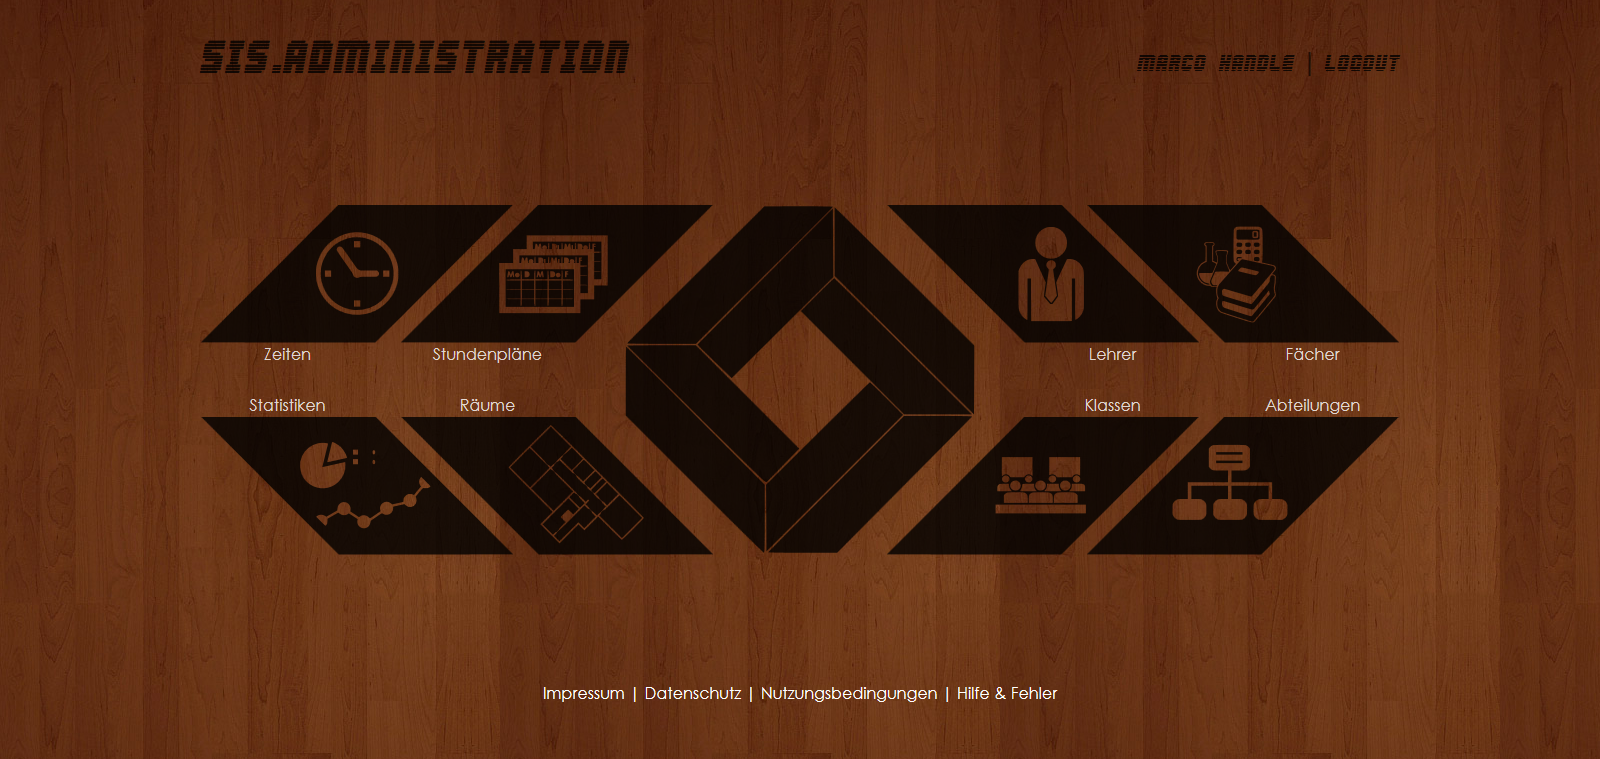
\includegraphics[keepaspectratio=true, width=17cm]{images/screenshots/admin_menu.png}
\caption{Administrationsmenü}
\label{fig:instr_other_menu}
\end{figure}
\subsection{Stunden}
Sollte es aus irgendeinem Grund dazu kommen, dass es mehr Stunden gibt oder sich die Start- und End-Zeiten der Stunden ändern kann dies hier vorgenommen werden.\\
Aus Sicherheitsgründen können Stunden nicht gelöscht werden, da es bei unabsichtlichem dazu kommt, dass die ganze Stundenpläne und Supplierpläne nicht mehr funktionieren. Deshalb eben diese Sicherheitsmaßnahme.\\
Die Eingabe ist so aufgebaut, dass man mit den Buttons rechts und links den Wochentag auswählen kann. Hat mn den Wochentag ausgewählt, so sind die Stunden dieses Wochentages zu sehen. Alle Felder sind bei einer neuen Stunde einzutragen, d.h. es muss jedes Feld ausgefüllt werden. Die Eingabemaske (siehe \autoref{fig:instr_other_hours}) sieht so aus, dass das Erste Feld den Namen der Stunde, nummerisch nummeriert, angibt. Dann kommt die Start-Zeit und anschließend die End-Zeit. Zum Abschluss muss Übernehmen geklickt werden.\\
Das löschen ist, wie oben beschrieben, nicht möglich, jedoch das verändern von vorhandenen Stunden ist möglich. 
\begin{figure}[H]
\centering
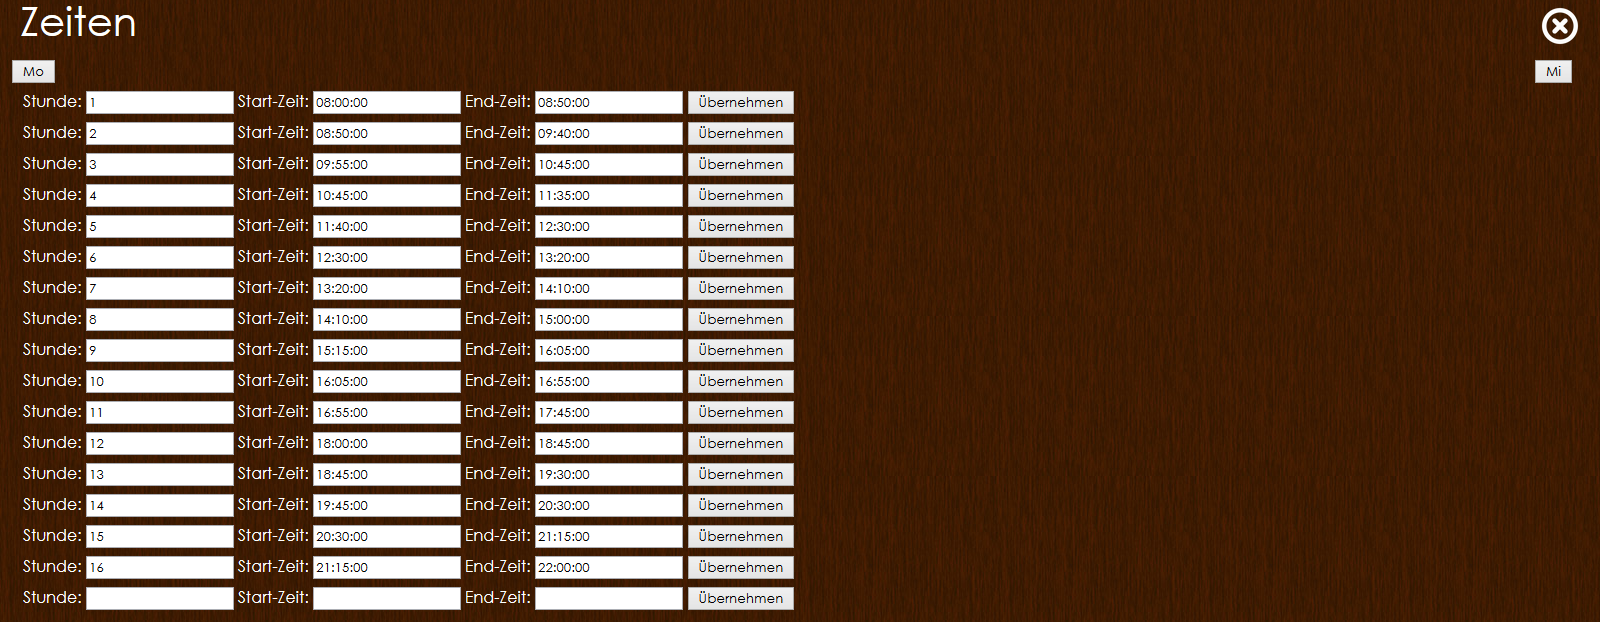
\includegraphics[keepaspectratio=true, width=17cm]{images/screenshots/hours_input.png}
\caption{Stunden bearbeiten}
\label{fig:instr_other_hours}
\end{figure}
\subsection{Stundenpläne}
Stundenpläne werden in dieser Eingabe eingegeben werden. Dazu muss im zuerst erscheinenden Menü die Klasse ausgewählt werden. Der Tag muss nicht ausgewählt werden, wird er nicht ausgewählt, so startet die Eingabe am Montag. Will man jedoch an einem spezifischen Tag die Eingabe beginnen, so muss man das Kürzel des Wochentages eingeben. Zum bestätigen muss auf OK geklickt werden. (Menü siehe \autoref{fig:instr_other_timetables_menu})
\begin{figure}[H]
\centering
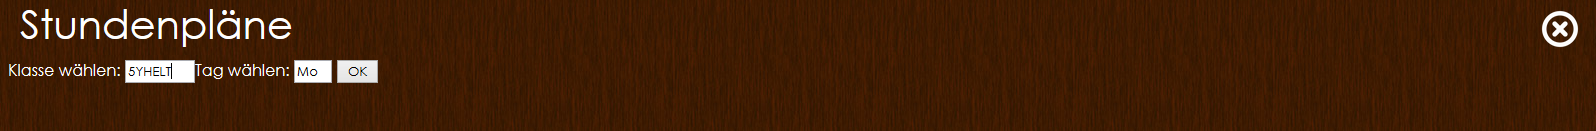
\includegraphics[keepaspectratio=true, width=17cm]{images/screenshots/timetables_input_menu.png}
\caption{Stundenplan auswählen}
\label{fig:instr_other_timetables_menu}
\end{figure}
Ist dies ausgewählt so gelangt man zur Eingabe der gewählten Klasse und des gewählten Tages. Im linken oberen Bereich des Fensters sind die gewählte Klasse und der gewählte Tag zu sehen. Mit einem Klick auf die Klasse gelangt man wieder ins Menü für die Klassenauswahl zurück. (siehe \autoref{fig:instr_other_timetables_infos})
\begin{figure}[H]
\centering
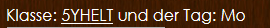
\includegraphics[keepaspectratio=true, width=6cm]{images/screenshots/timetables_input_infos.png}
\caption{Klasse und Tag}
\label{fig:instr_other_timetables_infos}
\end{figure}
Den Tag kann man mit den Buttons, welche links und rechts zu sehen sind, auswählen.  Mit einem Klick auf den Button wechselt man zu dem Tag, der auf dem Button zu sehen ist. (siehe \autoref{fig:instr_other_timetables_infos})
\begin{figure}[H]
\centering
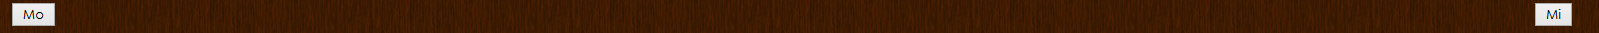
\includegraphics[keepaspectratio=true, width=17cm]{images/screenshots/timetables_input_day.png}
\caption{Tagauswahl}
\label{fig:instr_other_timetables_infos}
\end{figure}
Die Eingabemaske sieht wie in \autoref{fig:instr_other_timetables_layout} zu sehen ist aus. In den nächsten Abschnitten werden verschiedene Eintragungen beschrieben und somit auch die Eingabemaske beschrieben.
\begin{figure}[H]
\centering
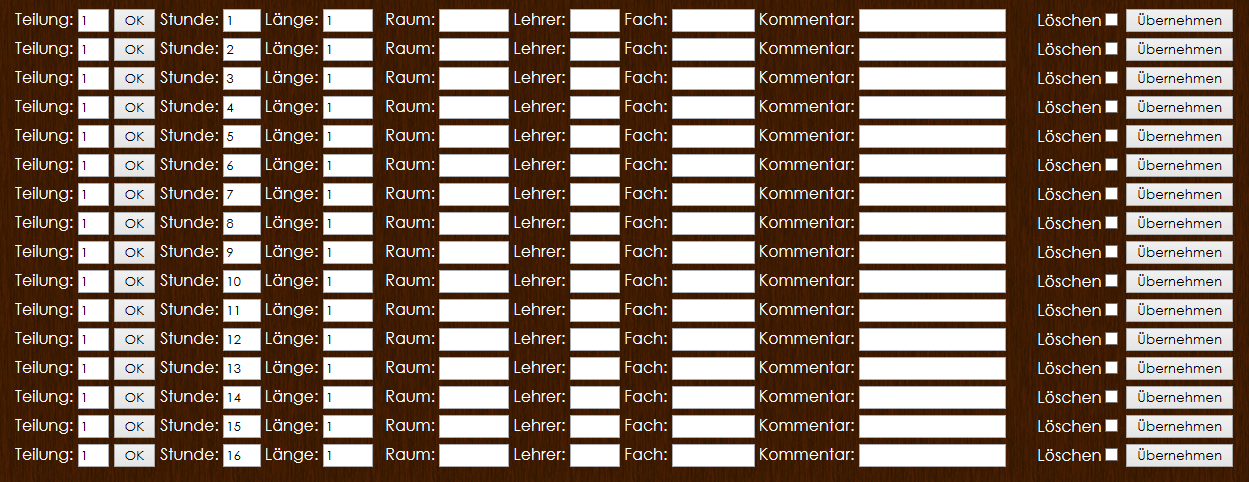
\includegraphics[keepaspectratio=true, width=17cm]{images/screenshots/timetables_input_layout.png}
\caption{Tagauswahl}
\label{fig:instr_other_timetables_layout}
\end{figure}
\subsubsection{Einzelstunde}
Soll eine Stunde eingetragen werden, welche nur eine Stunde lang ist, so muss an der Standardeinstellung nichts geändert werden. Es muss nur das Fach und der Lehrer eingetragen werden. In der zweiten Spalte ist die Stunde zu sehen. Will man in der zweiten Stunde eine Stunde hinzufügen, so muss dort eingetragen werden wo bei der Stunde 2 steht. Hat man die Stunde fertig eingetragen so muss man auf Übernehmen klicken. (Siehe Beispiel in \autoref{fig:instr_other_timetables_singleHour})
\begin{figure}[H]
\centering
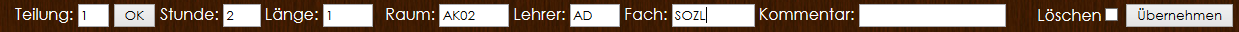
\includegraphics[keepaspectratio=true, width=17cm]{images/screenshots/timetables_input_singleHour.png}
\caption{Beispiel Einzelstunde}
\label{fig:instr_other_timetables_singleHour}
\end{figure}
\subsubsection{Mehrstündige Stunden}
Wenn eine Stunde eingetragen werden soll, die mehr als eine Stunde andauert, so muss dies in der Eingabemaske, dementsprechend vermerkt werden. Dies geschieht in der Textbox Länge. Beginnt die Stunde in der ersten Stunde und dauert 3 Stunden, so muss in der Zeile, in der bei Stunde 1 steht, bei Länge 3 eingefügt werden. Klickt man nun in eine andere Textbox, so werden die Stunden ausgeblendet, die durch die Länge nicht mehr benötigt werden. In diesem Beispiel wird die Stunde 2 und 3 ausgeblendet. Die restlichen eingaben funktionieren nach dem selben Prinzip, wie bei der Einzelstunde. (Siehe Beispiel in \autoref{fig:instr_other_timetables_multiHour})
\begin{figure}[H]
\centering
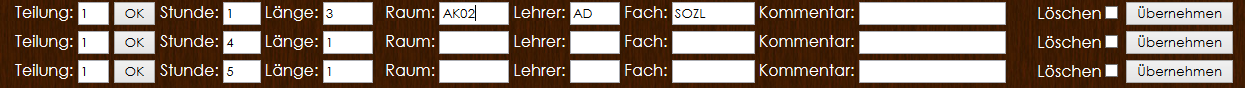
\includegraphics[keepaspectratio=true, width=17cm]{images/screenshots/timetables_input_multiHour.png}
\caption{Beispiel Mehrstündige Stunden}
\label{fig:instr_other_timetables_multiHour}
\end{figure}
\subsubsection{Teilungen}
Da es auch vorkommt, dass eine Klasse in sich geteilt wird, kann auch dies eingegeben werden. Dazu ist die Textbox Teilung zuständig. Dies funktioniert nur wenn die geteilten Fächer genau gleich lang sind. Sind sie unterschiedlich lang, so muss es anders eingegeben werden. Ist die Klasse in sich einmal geteilt und eine Hälfte hat 2 Stunden und die andere Hälfte 3 Stunden Unterricht, so muss die Teilung für die ersten 2 Stunden eingetragen werden und die andere Stunde kann als einzelne Stunde eingetragen werden.\\
Soll nun eine Teilung eingegeben werden, muss zuerst die Anzahl der Teilungen eingegeben werden und anschließend auf OK geklickt werden. Anschließend erscheinen weitere Zeilen. Die maximale Teilung die eingetragen werden kann ist 7 Teilungen. (siehe \autoref{fig:instr_other_timetables_divide7}) Die Länge der Stunde kann gleich wie bei keiner Teilung eingestellt werden.
\begin{figure}[H]
\centering
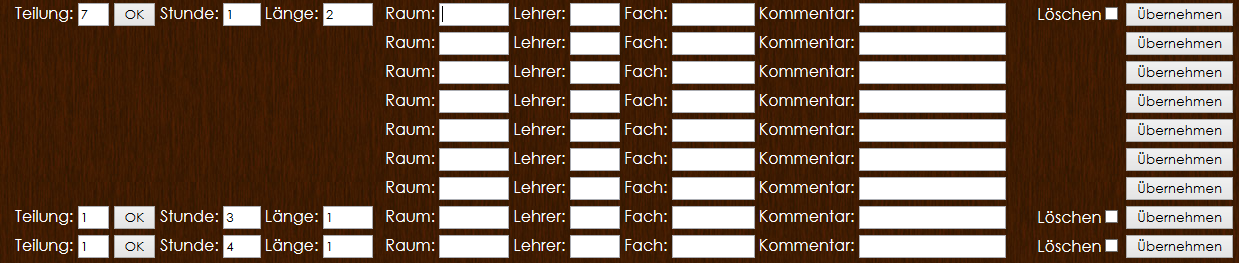
\includegraphics[keepaspectratio=true, width=17cm]{images/screenshots/timetables_input_divide7.png}
\caption{Beispiel Mehrstündige Stunden}
\label{fig:instr_other_timetables_divide7}
\end{figure}
Jede eigene Zeile muss mit Übernehmen bestätigt werden. Gelöscht kann jedoch nur ein ganzer Block werden. Dies muss mit einem Hacken bei Löschen und anschließendem klicken auf Übernehmen erfolgen.
\subsubsection{Löschen}
Es können prinzipiell ganze Stundenblöcke gelöscht werden, jedoch gibt es noch die Möglichkeit den ganzen Tag dieser Klasse zu löschen. Dies geschieht mit dem Button links oben. (siehe \autoref{fig:instr_other_timetables_delete}) Klickt man auf diesen Button werden die Stunden dieser Klasse und dieses Tages unwiderruflich gelöscht.
\begin{figure}[H]
\centering
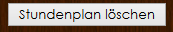
\includegraphics[keepaspectratio=true, width=5cm]{images/screenshots/timetables_input_delete.png}
\caption{Beispiel Mehrstündige Stunden}
\label{fig:instr_other_timetables_delete}
\end{figure}
\subsection{Lehrer}
ad
\subsection{Fächer}
asd
\subsection{Statistiken}
asd
\subsection{Räume}
asd
\subsection{Klassen}
asd
\subsection{Abteilungen}
ad